\section{Minimal stretch factors for non-orientable surfaces with marked points}
\label{sec:application}

In this section we will use \autoref{thm:classifying-fibrations} and Proposition  \ref{prop:asymptotic} to adapt the methods of Yazdi \cite{yazdi2018pseudo} to non-orientable surfaces. We recall the statement of the main theorem:
\begin{manualtheorem}
  {\ref{thm:stretch1}}
Let $\no_{g,n}$ be a non-orientable surface of genus $g$ with $n$ punctures, and let $\ell_{g,n}'$ be the logarithm of
  the minimum stretch factor of the pseudo-Anosov mapping classes acting on $\no_{g,n}$.
  Then for any fixed $n \in \mathbb{N}$, there is a positive constant $B'_1 = B'_1(n)$ and $B'_2 = B'_2(n)$ such
  that for any $g \geq 3$,
  %\becca[inline]{This should be 3, right?  When we are talking about non-orientable genus?}
  %\sayantan[inline]{Yes, that is correct. I have made the changes elsewhere in the document to reflect this correction.}
  the quantity $\ell_{g,n}'$ satisfies the following inequalities:
  \begin{align*}
    \frac{B'_1}{g} \leq \ell'_{g,n} \leq \frac{B'_2}{g}.
  \end{align*}
\end{manualtheorem}


%Recall that associated to every pseudo-Anosov homeomorphism $f$ there is a number $\lambda(f)$, the
%\textit{dilatation} or \textit{stretch factor}, the amount that the stable and unstable foliations of the
%pseudo-Anosov change by. Given a surface $S$, it is natural to ask what we can say about the set of all
%possible stretch factors, i.e.
%\begin{align*}
%    \left\{\log(\lambda(f)) \mid f \in \text{Mod}(S) \text{ is pseudo-Anosov}\right\}
%\end{align*}

%We call this set the \textit{spectrum} of $S$. A first step at understanding this set of all stretch factors associated to a surface is considering the following quantity
%\begin{align*}
%    l_{g,n} =\min\{\log(\lambda(f)) \mid f \in \text{Mod}(\mathcal{S}_{g,n}) \text{ is pseudo-Anosov}\}.
%\end{align*}

%The study of this minimal stretch factor $l_{g,n}$ was initiated by Penner in his work
%\cite{penner1991bounds}. In this paper Penner studied the asymptotic behavior of minimal stretch factors of orientable surfaces without punctures, i.e. the behavior of $l_{g,0}$. He showed that there exist positive constants
%$A_1$ and $A_2$ such that the following inequalities held for any $g \geq 2$.
%\begin{align*}
%    \frac{A_1}{g} \leq l_{g,0} \leq \frac{A_2}{g}
%\end{align*}
%This showed that asymptotically $l_{g,0}$ behaves like $\frac{1}{g}$ for $g \geq 2$.
%It turns out something similar is true when one starts adding punctures. Yazdi showed
%that for any fixed $n$, $l_{g,n}$ behaves like $\frac{1}{g}$. More precisely, he proved the following theorem.
%\begin{thm}[Theorem 1.2 of \cite{yazdi2018pseudo}]
%\label{thm:yazdi1}
%For any fixed $n \in \mathbb{N}$, there are positive constants $B_1 = B_1(n)$ and $B_2 = B_2(n)$ such that the following inequalities hold for
%any $g \geq 2$.
%\begin{align*}
%    \frac{B_1}{g} \leq l_{g,n} \leq \frac{B_2}{g}.
%\end{align*}
%\end{thm}

%Yazdi's result is one of many recent results in studying the asymptotics of $l_{g,n}$ for different subsets of
%the $(g,n)$ plane. See the introductions of \cite{yazdi2018pseudo} and \cite{tsai2009asymptotic} for more
%examples of results of this form. 

%Yazdi proves an additional result along these lines for a large subset of
%the $(g,n)$ plane, one containing balls of arbitrary large radii.

%\begin{thm}[Yazdi]
%    \label{thm:yazdi2}
%    There exists positive constants $A$, $B$ and $C$ such that for any $n \geq 1$ and $g \geq Cn\log^2(n)$ such that
%    the following inequalities hold.
%    \begin{align*}
%        \frac{B}{g} \leq l_{g,n} \leq \frac{A}{g}
%    \end{align*}

%\end{thm}

%A key tool in Yazdi's proof of this theorem is the fibered face theory of Thurston. With the non-orientable analog of
%Thurston's fibered face theory we developed in the previous section, it's possible to prove an analogous
%theorem for non-orientable punctured surfaces.  Let $\mathcal{N}_{g,n}$ be the genus $g$ non-orientable
%surface with $n$ punctures and let $l_{g,n}'$ be the minimal stretch factor of $\no_{g,n}$.
%\begin{align*}
%  l'_{g,n} = \min\left\{\log(\lambda(f)) \mid f \in \text{Mod}(\mathcal{N}_{g,n})\ \text{is pseudo-Anosov}\right\}
%\end{align*}
%Then we have the following result, analogous to Yazdi's results.
%\begin{thm}
%  \label{thm:stretch1}
%  For any fixed $n \in \mathbb{N}$, there are positive constants $B'_1 = B'_1(n)$ and $B'_2 = B'_2(n)$ such that
%  for any $g \geq 2$, the stretch factor satisfies the following inequalities.
%  \begin{align*}
%    \frac{B'_1}{g} \leq l'_{g,n} \leq \frac{B'_2}{g}
%  \end{align*}
%\end{thm}

Observe that the lower bound for the non-orientable case follows easily from the lower bound for the orientable case.
Indeed, let $\varphi$ be a pseudo-Anosov map with the minimal stretch factor on $\no_{g,n}$. The orientation double cover of $\no_{g,n}$ is $\os_{G-1,2n}$ where $G=2g$.  Note that in the non-orientable case we measure genus as the number of copies of the projective plane attached to $S^2$ via a connect sum and in the orientable case we measure genus as the number of copies of the torus attached to $S^2$ via a connected sum. Let $\wt{\varphi}:\os_{G-1, 2n}\to\os_{G-1,2n}$ be the orientation preserving lift of $\varphi$.
By Proposition \ref{prop:2}, $\wt{\varphi}$ has the same
stretch factor as $\varphi$. The former is bounded below by $\frac{B_1}{G-1}$, and thus the stretch factor of $\varphi$ is bounded
below as well. The more challenging part of the proof is showing that the upper bound holds. %We will constructing pseudo-Anosov maps with small stretch factors, adapting Yazdi's techniques to the non-orientable setting.

We will closely follow Yazdi's construction, which proceeds in five steps that we will reorder for clarity.  In steps 1 and 2, we construct a family of psuedo-Anosov homeomorphisms
of $\no_{g_i,n}$, where $\{g_i\}$ is an unbounded increasing sequence. However the sequence $\{g_i\}$ does not contain all natural numbers.  In step 3 we gives an upper bound to the stretch factor of the previously constructed homeomorphisms. In steps 4 and 5, we construct pseudo-Anosov maps on surfaces of genera that do not belong to the sequence $\{g_i\}$. It is in steps 4 and 5 that we uses
Thurston's fibered face theory. We have adapted  each of Yazdi's five steps to work for non-orientable surfaces.

\p{Step 1: Constructing the surfaces}
%We first construct surfaces with rotational symmetry. Using this symmetry, if one shows that a power of some homeomorphism is pseudo-Anosov, then so is the original homeomorphism \cite{penner1991bounds}.

%We will try to follow Yazdi's notation as close as we can, in order to make it clear to the reader
%how our construction replicates his.

We begin by defining a family of surfaces $P_{n,k}$. Let $S$ be an orientable surface of genus 5 with 3
boundary components.  Call the boundary components $c,d$ and $e$. Choose an orientation of $S$ and let $c,d$ and $e$ inherit the induced orientations. We obtain a non-orientable surface $T$ from $S$ by adding two cross caps to $S$ (retaining the orientation of the boundary components of $S$). Let $p$ and $q$ be marked points in the boundary component $e$. In Step 5 we will remove $p$ and all copies.  Let  $r$ and
$s$ be the components of $e\setminus\{p,q\}$. The resulting surface $N$ is shown in \autoref{fig:buildingblock}.

\begin{figure}[ht]
    \centering
    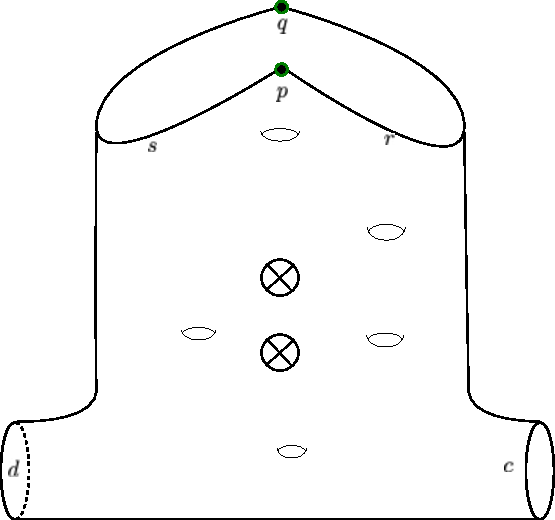
\includegraphics[scale=0.8]{t.pdf}
    \caption{The surface $T$, which will be the building block of the construction.}
    \label{fig:buildingblock}
\end{figure}

Let $T_{i,j}$ be copies of the surface $T$, where $i,j \in \mathbb{Z}$. Let $c_{i,j}, d_{i,j}$ and $e_{i,j}$ be the (oriented) boundary components of $T_{i,j}$ and let $r_{i,j}$ and $s_{i,j}$ be the copies of the arcs $r$ and $s$ in $T_{i,j}$. Define a connected infinite surface $T_\infty$ as the quotient:
\begin{align*}
  T_\infty \coloneqq \left. \left( \bigcup T_{i,j} \right)\right/\sim
\end{align*}
for all integers $i$ and $j$. The gluing $\sim$ is given by orientation-reversing identifications:
\begin{align}
\label{identification}
  c_{i,j} &\sim d_{i+1,j} \\
  r_{i,j} &\sim s_{i,j+1}.
\end{align}
%where the boundary components are glued by an orientation-reversing homeomorphism.


We have two
natural shift maps $\overline{\rho_1},\overline{\rho_2}: T_\infty \to T_\infty$ that act in the
following manner:
\begin{align*}
  \overline{\rho_1}: T_{i,j} &\mapsto T_{i+1, j} \\
  \overline{\rho_2}: T_{i,j} &\mapsto T_{i, j+1}.
\end{align*}

Note that $\overline{\rho_1}$ and $\overline{\rho_2}$ commute. Define the surface $P_{n,k}$ as the quotient of the surface $T_\infty$ by the
covering action of the group generated by $(\overline{\rho_1})^n$ and $(\overline{\rho_2})^k$. Then
$\overline{\rho_1}$ and $\overline{\rho_2}$ are equivariant with respect to the covering map.  We denote the induced homeomorphisms of the quotient $P_{n,k}$ by $\rho_1$
and $\rho_2$.  Note that later we will require that $k\geq 3$ and $n$ is the number of punctures, given in \autoref{thm:stretch1}.

%We use the surface $T$ as the building blocks for two reasons:
%\begin{itemize}
%\item The combinatorics of the curves in \autoref{fig:curves} make the associated matrix from the Penner construction satisfy the conditions of Lemma \ref{lem:spectral}. This is used to prove our family of pseudo-Anosov maps have stretch factors bounded above by the quantity we desire.
%\item We will construct a pseudo-Anosov homemorphism $\varphi$ of $T$\becca[inline]{this previously referenced ``a given pseudo-Anosov."  We mean of $T$, right?} such that $\gamma$ and $\varphi(\gamma)$ we construct form the boundary of an embedded $\RR P^2$ with two boundary components in the mapping torus, which will come into play when extending our family of surfaces in Step 3.
%\end{itemize}

\begin{lem}
\label{lem:genera}
Let
\begin{align*}
    g_{n,k} &= (14k - 2)n + 2
\end{align*} for $n \geq 1$ and $k \geq 1$.
    The genus of $P_{n,k}$ is $g_{n,k}$.
\end{lem}
\begin{proof}
%Let $U$ be the quotient of $P_{n,k}$ by the subgroup of $\Mod(P_{n,k})$ generated by $\overline{\rho}_1$.  Therefore $P_{n,k}$ is a $n$-fold cover of $U$.  Because $\overline{\rho}_1$ and $\overline{\rho}_2$ commute, the quotient of $T_\infty$ by $\langle \overline{\rho}_1,\overline{\rho}_2^k$ induces a covering space of $T_\infty$ over $U$.  Let $\pi$ be the covering map $T_\infty\rightarrow U$.  Then $\pi$ is also the composition of the covering map of $T_\infty\to P_{n,k}$ and the covering space of $P_{n,k}\to T_\infty$. Moreover, because $\overline{\rho}_1$ is a deck transformation of $\pi$, each $T_{i,j}$ is a fundamental domain of $\pi$.  The map $\pi$ identifies the boundary components $c_{i,j}$ and $d_{i,j}$ and the arcs $r_{i,j}$ and $s_{i,j}$.  Therefore $\chi(U)=\chi(T_{i,j})=2-% The deck group of the covering space of $T_\infty$ over $U$ is 
  Let $U \subset P_{n,k}$ be the subsurface
  \begin{align*}
    U = \left. \left( \bigcup_{j =0}^{k-1} T_{0,j} \right)\right/\sim'
  \end{align*}
  where $\sim'$ is given by (\ref{identification}) and by identifying $r_{i,k-1}$ and $s_{i,0}$.
  Then $U$ is a compact, non-orientable surface of genus $12k$ with $2k$ boundary components.  %Moreover, $U$ is a fundamental domain for the covering action of $rho_1$ on $T_\infty$. 
  %We can compute the Euler characteristic of $U$: %in order to determine the Euler characteristic of $P_{n,k}$:
  %\begin{align*}
  %  \chi(U) &= 2 - 12k - 2k \\
  %          &= 2 - 14k.
  %\end{align*}
  %Since $P_{n,k}$ is formed by identifying $c_{i,j}$ with $d_{i+1,j}$ for $0\leq i\leq n-1$ and $c_{n-1,j}$ with $d_{0,j}$ for all $j$, 
  The surface $P_{n,k}$ consists of $n$ copies of $U$ identified along the $2k$ boundary components.  Therefore the Euler characteristic of $P_{n,k}$ is:
  \begin{align*}
    \chi(P_{n,k}) &= n \cdot \chi(U)\\
                  &=n\cdot(2-12k-2k)\\
                  &= -n(14k - 2).
  \end{align*}
  Since $P_{n,k}$ is a non-orientable surface with empty boundary, we have that:
  \begin{align*}
    g_{n,k} = n(14k-2) + 2.
%    \vspace{-30pt}
  \end{align*}
\end{proof}

\p{Step 2: Constructing the maps}
In what is now a classical paper, Penner gives a construction of pseudo-Anosov homeomorphisms both orientable and non-orientable surfaces \cite{penner1988construction}.  Below we outline the Penner construction for non-orientable surfaces following the details of Liechti--Strenner \cite[Section 2]{LS}.

%\p{The Penner construction} Let $S$ be an orientable surface.  Let $A = \{a_1,\dots,a_n\}$ and $B = \{b_1,\dots,b_m\}$ be multicurves in $S$.  A Penner construction is mapping class given as a composition of Dehn twists that satisfy the following:
%\begin{enumerate}
%\item the complement of $A\cup B$ in $N$ consists of disks with at most one puncture or marked point,
%    \item a Dehn twist about each curve in $A\cup B$ is included in the composition,
%    \item each Dehn twist about a curve in $A$ is a left-handed Dehn twist, and
%    \item each Dehn twist about a rurve in $B$ is a right-handed Dehn twist.
%\end{enumerate}
%  A set of curves that satisfies the first condition is said to {\it fill} $S$.  Penner proves that this construction is pseudo-Anosov \cite{penner1988construction}.
%
% However, for non-orientable surfaces, there is not a well-defined notion of a left or right Dehn twist. Therefore we use the notion of an inconsistent marking, as follows.

 \p{Inconsistent markings} Let $\no$ be a non-orientable surface and let $c$ be a two-sided curve in $\no$.  There exists a neighborhood of $c$ that is homeomorphic to an annulus.  Let $\mathcal{A}_c$ be an annulus and let $\zeta_c: \mathcal{A}_c \xrightarrow{} \no$ be the homeomorphism that maps to a neighborhood of $c$.  The homeomorphism $\zeta_c$ is called a \textit{marking} of $c$. A pair consisting of a curve $c$ and $\zeta_c$ is called a {\it marked curve}.  
 If we fix an
orientation of $\mathcal{A}_c$, then we can pushforward this orientation to $\no$. Let
$(c,\zeta_c)$ and let $(d,\zeta_d)$ be two marked curves that intersect at one point $p$.  We say that $(c,\zeta_c)$ and $(d,\zeta_d)$ are {\it marked inconsistently} if the
pushforward of the orientation of $\mathcal{A}_c$ and disagrees with the pushforward of the orientation of $\mathcal{A}_d$ in a neighborhood of $p$.  We emphasize that we can also say that two disjoint curves are inconsistently marked.

\p{Dehn twists} We define the Dehn twist $\phi_{c,\zeta_c}(x)$ around a marked curve $(c,\zeta_c)$ as:
\begin{align*}
  \phi_{c,\zeta_c}(x) =
  \begin{cases}
    \zeta_c \circ \tau_c \circ \zeta_c^{-1}(x) & \text{for } x \in \zeta_c(\mathcal{A}_c) \\
    x & \text{for } x \in \no - \zeta_c(\mathcal{A}_c)
  \end{cases}.
\end{align*}
Here $\tau_c$ is the left-handed Dehn twist on $\mathcal{A}_c$, i.e. $\tau_c(\theta,t) = (\theta + 2\pi t,t)$. 

\p{The Penner construction for non-orientable surfaces} Let $\mathcal{C}$ be a set of marked essential simple closed curves in $\no$ such that no two curves in $\mathcal{C}$ are homotopic.  A Penner construction on $\no$ is a composition of Dehn twists about the marked curves in $\mathcal{C}$ such that:
\begin{enumerate}
\item the complement of curves in $\mathcal{C}$ in $\no$ consists of disks with at most one puncture or marked point,
    \item the marked curves $(c_i,\zeta_i),(c_j,\zeta_j)\in\mathcal{C}$ with $i\neq j$ are marked inconsistently,
    \item a Dehn twist about each marked curve in $\mathcal{C}$ is included in the composition, and
    \item all powers of Dehn twists are positive (alternatively, all powers are negative).
\end{enumerate}

%If the set $\mathcal{C}$ satisfies the first condition, it is said to {\it fill} $\no$.


%\caleb[inline]{Alright, so we actually discuss the subspace spanned by the transverse measures specific to our set of curves in the proof of Lemma 4.3. And I think that's enough for our purposes, so I added some of the text below to the beginning of Step 4. I think it sounds a little awkward though.}

%\p{Train tracks} Penner not only proved that mapping classes constructed by the Penner construction are pseudo-Anosov, he also determines their stretch factor (see \cite{penner1988construction}).  %The proof that the Penner construction on non-orientable surfaces is pseudo-Anosov, and the computation of stretch factor are the same as in the orientable setting.  Let $\varphi$ be a pseudo-Anosov homeomorphism of $\no$.  A {\it train track} is an embedded graph in $\no$ such that for every vertex $v$ of valence three or greater, all edges adjacent to $v$ have the same tangent vector at $v$.  An {\it invariant train track for $\varphi$} is a train track track $\tau$ such that $\varphi(\tau)$ is homotopic to $\tau$.  Let $\mathcal{C}$ be a collection of curves in $\no$. %Consider now the collection of transverse measures on our train track $\tau$.  For every curve $\gamma \in\mathcal{C}$,\becca[inline]{Do we need a condition on $\mathcal{C}$?  Filling, maybe?} there is an associated transverse measure $\mu_\gamma$ for $\tau$ that assigns $1$ to all edges lying in $\gamma$ and 0 to everything else. Let $V_\tau$ be the cone of transverse measures on $\tau$, and $H$ the subspace of $V_\tau$ spanned by the transverse measure associated to curves in $\mathcal{C}$.
%%\begin{align*}
 %% H = \mathrm{span}(\{\mu_\gamma \mid \gamma \text{ is a connected curve in } \mathcal{C}\}).
%%\end{align*}
%The measures $\mu_\gamma$ are linearly independent and form the \textit{standard basis} for $H$. The subspace $H$ is invariant under the action of $\varphi$ on $V_\tau$, thus $\varphi$ has a linear action on $H$. If we let $M$ be the matrix representing this action in the standard basis, then the stretch factor of $\varphi$, $\lambda(\varphi)$, is the Perron-Frobenius eigenvalue of $\varphi$.

\p{Construction of $f_{n,k}$} We now construct homeomorphisms $f_{n,k}: P_{n,k} \to P_{n,k}$ that are defined as a composition of specific Dehn twists
followed by a finite order mapping class. The key insight is that a power of this map will be a composition of
Dehn twists that satisfy the criteria to be a Penner construction.\becca[inline]{Is it a power or the actual map?}  Therefore $f_{n,k}$ is pseudo-Anosov. Here we are using the rotational symmetry of the $P_{n,k}$.

\begin{figure}[t]
    \centering
    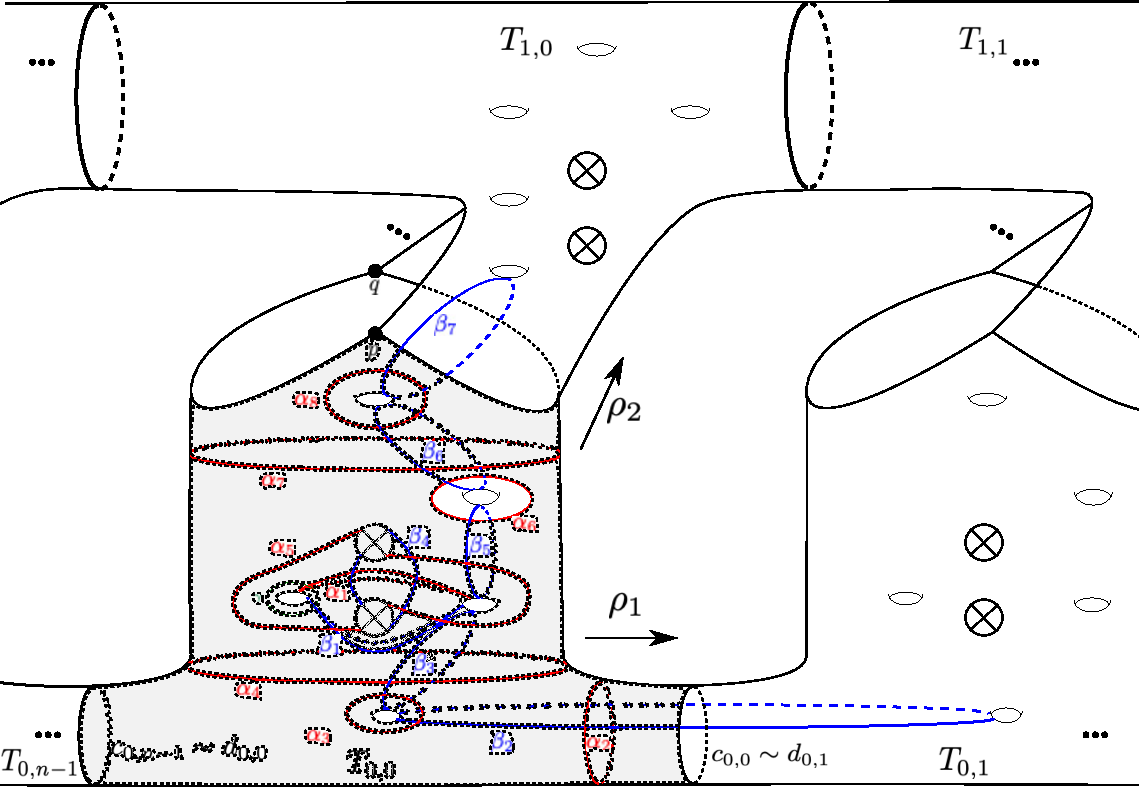
\includegraphics[scale=0.6]{surfaces1}
    \caption{Part of surface $P_{n,k}$ that includes the subsurface $T_{0,0}$ and the curves $\alpha_i$, $\beta_j$, and $\gamma$.}
    \label{fig:curves}
\end{figure}

%\begin{figure}[t]
 %   \centering
 %   \incfig[0.4]{ExtraCurves}
%    \caption{The parts of curves $\beta_2$ and $\beta_7$ on $T_{0,1}$ and $T_{1,0}$}
 %   \label{fig:extracurves}
%\end{figure}

%Recall that for non-orientable surfaces, we did not initially have a well-defined notion of a positive or negative Dehn twist. As we saw in \autoref{sec:backgr-mapp-class}, in order to use the Penner construction to construct pseudo-Anosov mapping classes, we need to ensure that the curves about which we twist are marked inconsistently. 
Let $\{\alpha_1,\cdots,\alpha_8\}$ be the multi-curve in $T_{0,0}$ as shown in \autoref{fig:curves}.  Let $\{\beta_1,\cdots,\beta_7\}$ be the multi-curve in $T_{0,0}\cup T_{0,1}\cup T_{1,0}$ shown in \autoref{fig:curves}. % All intersections of curves in $\{\alpha_1,\cdots,\alpha_8\}$ and $\{\beta_1,\cdots,\beta_7\}$ are shown in \autoref{fig:curves}.

For any $\alpha_i$, we choose a marking $\zeta_{\alpha_i}$ to be orientation-preserving.  For any $\beta_j$ let $\zeta_{\beta_j}$ be
orientation reversing. From here forward, we will think of $\alpha_i$ and $\beta_j$ as (inconsistently) marked curves but we will suppress the marking maps. These choices give an inconsistent marking of $\{\alpha_1,\cdots,\alpha_8\}\cup\{\beta_1,\cdots,\beta_7\}$.

Let 
$$\mathcal{R}=\displaystyle\bigcup_{i=2}^8\alpha_i.$$ Then $\mathcal{R}$ is a marked multi-curve that is disjoint from $\gamma$.  Let
$$\overline{\mathcal{R}}= \mathcal{R} \cup \rho_1(\mathcal{R}) \cup \dots \cup
\rho_1^{n-1}(\mathcal{R}).$$
Let $\Phi_r$ be the composition of Dehn twists about the marked curves in $\overline{\mathcal{R}}$.  Because the curves in $\overline{\mathcal{R}}$ are disjoint, the Dehn twists about the curves commute.

Let $$\mathcal{B}=\displaystyle\bigcup_{j=2}^7\beta_j$$ in $T_{0,0} \cup T_{0,1} \cup T_{1,0}$. As above, $\mathcal{B}$ is a marked multi-curve that is disjoint from $\gamma$.  Let $$\overline{\mathcal{B}} = \mathcal{B} \cup \rho_1(\mathcal{B}) \cup \dots \cup
\rho_1^{n-1}(\mathcal{B}).$$
Let $\Phi_b$
as the composition of Dehn twists about all of the marked curves in $\overline{\mathcal{B}}$.
As with $\overline{\mathcal{R}}$, the Dehn twists about curves in $\overline{\mathcal{B}}$ 
commute.




Let $\alpha_1,\beta_1 \subset T_{0,0}$ be the (marked) curves in \autoref{fig:curves}. Let $\Phi$ be the composition
of Dehn twists along all the curves $\alpha_1, \rho_1(\alpha_1), \dots, \rho_1^{n-1}(\alpha_1)$ followed by
Dehn twists along all the curves $\beta_1,\rho_1(\beta_1),\dots,\rho_1^{n-1}(\beta_1)$. Define the map $f_{n,k}$
as:
\begin{align*}
    f_{n,k} &\coloneqq \rho_2 \circ \Phi \circ \Phi_b \circ \Phi_r
\end{align*}
Since the curves about which we twist to construct $f_{n,k}$ satisfy the conditions of Penner's construction, $f_{n,k}$ is a pseudo-Anosov homeomorphism.%It follows from the Penner construction that $(f_{n,k})^k$ is pseudo-Anosov.% Hence $f_{n,k}$ itself is pseudo-Anosov and an invariant train track $\tau_{n,k}$ for $f_{n,k}$ can be obtained from Penner's construction that we described in \autoref{sec:backgr-mapp-class}.

\p{Step 3: Bounding the Stretch Factor}
Following Yazdi, our next goal is to find an upper bound for the stretch factor of the pseudo-Anosov homeomorphisms $f_{n,k}$.
%Yazdi then finds an upper bound for the logarithm of the stretch factors of the pseudo-Anosov homeomorphisms he constructed. Similarly, we want to find an upper bound for the homeomorphisms we constructed in Step 2.  

\p{Train tracks} Let $S$ be a surface.  A \textit{train track} in $S$ is graph embedded in $S$ with that property that for every vertex $v$ of valence three or greater, all edges adjacent to $v$ have the same tangent vector at $v$. Let $\varphi:S\rightarrow S$ be a pseudo-Anosov homeomorphism.  The map $\varphi$ is equipped with a train track whose image under $\varphi$ is homotopic to itself.  Such a train track is an \textit{invariant train track} associated to $\varphi$. Invariant train tracks have an associated matrix whose Perron-Frobenius eigenvalue is the stretch factor of $\varphi$.

%recall in \autoref{sec:backgr-mapp-class} we saw that pseudo-Anosov maps give rise to matrices whose Perron-Frobenius eigenvalue isthe corresponding stretch factor. So a way to find an upper bound of the stretch factor of the maps we have constructed is to bound the spectral radius of the associated matrices. The following lemma by 

Yazdi uses the Lemma \ref{lem:spectral} to bound the spectral radius of the associated matrices.

\begin{lem}[Lemma 2.3 of \cite{yazdi2018pseudo}]
\label{lem:spectral}
Let $A$ be a non-negative integral matrix, $\Gamma$ be the adjacency graph of $A$, and $V(\Gamma)$ the set of
vertices of $\Gamma$. For each $v \in V(\Gamma)$, define $v^+$ to be the set of vertices $u\in V(\Gamma)$ such that there
is an oriented edge from $v$ to $u$. Let $D$ and $k$ be fixed natural numbers. Assume the following conditions
hold for $\Gamma$:
\begin{enumerate}[(i)]
\item For each $v \in V(\Gamma)$ we have $\deg_{\text{out}}(v) \leq D$,
\item There is a partition $V(\Gamma) = V_1 \cup \dots \cup V_\ell$ such that for each $v \in V_i$ we have
  $v^+ \subset V_{i+1}$, for any $1 \leq i \leq \ell$ except possibly when $i = 1$ or 3 (indices are mod $\ell$),
\item For each $v \in V_1$, we have $v^+ \subset V_2 \cup V_3$,
\item For each $v \in V_3$ we have $v^+ \subset V_3 \cup V_4$, and for $u \in v^+ \cap V_3$ we have
  $u^+ \subset V_4$, and 
\item For all $3 < j \leq k$ and each $v \in V_j$, the set $v^+$ consists of a single element.
\end{enumerate}

Then the spectral radius of $A^{\ell-1}$ is at most $4D^4$.

\end{lem}
\noindent With this result in hand, we can find an upper bound for the stretch factor of $f_{n,k}$

\begin{lem}\label{lem:upperbound}
  Let $\lambda_{n,k}$ be the stretch factor of $f_{n,k}$. Then there exists a universal positive constant $C'$ such that for every $n \geq 1$ and $k \geq 3$, we have the following upper bound on $\log(\lambda_{n,k})$.
  \begin{align*}
   \log(\lambda_{n,k}) \leq C'\frac{n}{g_{n,k}}
  \end{align*}
\end{lem}

\begin{proof}
 We deliberately constructed our curves so that all intersections of the multi-curve $\{\alpha_1,\dots,\alpha_8\}$ and $\{\beta_1,\dots,\beta_7\}$ occur in the subsurface $T_{0,0}$. The curve $\beta_3$ intersects $\rho_2(\alpha_3)$ at one point in $T_{0,1}$ and $\beta_7$ intersects $\rho_1(\alpha_8)$ at one point in $T_{1,0}$.

  We define the following unions of marked curves:
\begin{align*}
  \mathcal{A} &\coloneqq \mathcal{B} \cup \mathcal{R} \cup \{\alpha_1,\beta_1\} =\bigcup_{i=1}^8\alpha_i\cup\bigcup_{j=1}^7\beta_j\\
  \smallskip
  \overline{\mathcal{A}} &\coloneqq \mathcal{A} \cup \rho_1(\mathcal{A}) \cup \dots \cup \rho_1^{n-1}(\mathcal{A}) \\
  \widehat{\mathcal{A}} &\coloneqq \overline{\mathcal{A}} \cup \rho_2\left(\overline{\mathcal{A}}\right) \cup \dots \cup \rho_2^{k-1}\left(\overline{\mathcal{A}}\right).
\end{align*}

Because $f_{n,k}$ is pseudo-Anosov, it has a corresponding invariant train track $\tau$.
Let $V_{\tau}$ be the space of all measured foliations that can be obtained by varying the weights on the tracks of $\tau$.
This forms a finite dimensional cone of measures, all of which can be carried by the combinatorial train track $\tau$.
Furthermore, $f_{n,k}$ acts linearly on this cone, and leaves the cone invariant, since $\tau$ is an invariant track for $f_{n,k}$.
Consider now the transverse measure $\mu_{\delta}$ for any curve $\delta$ in $\widehat{\mathcal{A}}$.
This transverse measure is carried by $\tau$, and thus $\mu_{\delta}$ belongs in the cone of measures $V_{\tau}$.
Let $H$ be the subspace spanned by $\{\mu_\delta \mid \delta\subset\widehat{\mathcal{A}}\}$.
This linear subspace is also left invariant by $f_{n,k}$, so we can restrict our attention to the matrix of $f_{n,k}$ with respect to the basis
%\sayantan[inline]{What justification does Yazdi use to claim that this spanning set actually forms a basis?}
%\becca[inline]{``It's easy to see that the $\mu_x$ are indeed linearly independent."}
%\sayantan[inline]{I think that's alright then. We can leave it to the reader to check.}
given by the $\{\mu_\delta \mid \delta\subset\widehat{\mathcal{A}}\}$. Let $M$
be the matrix representing this linear action on $H$.  Let $\Gamma$ be the adjacency graph for $M$. Work of Penner \cite{penner1988construction} tells us that the Perron--Frobenius eigenvalue of $M$ is the stretch factor of $f_{n,k}$.
%Let $A$ be the matrix that $f_{n,k}$ on the subspace of the cone of transverse measures that is spanned by the measures assigning $1$ to single curves in $\widehat{\mathcal{A}}$ and 0 to everything else. Let $A$ be said matrix and $\Gamma$ the adjacency graph of $A$. 

%\sayantan[inline]{Rewrite this to be a little more comprehensible.}

To bound the spectral radius of $M$, we need to show that $\Gamma$ satisfies
the criteria of Lemma \ref{lem:spectral}.

%We can now check the conditions of Lemma \ref{lem:spectral}, based on the combinatorics of the curves on our surface:

\begin{enumerate}[(i)]
\item There exists a constant $D'$, independent of $n$ and
  $k$, such that for every curve $\delta \in \widehat{\mathcal{A}}$, the geometric
  intersection number between $\delta$ and every curve in $\overline{\mathcal{A}}$ is at most $D'$. %Recall from \autoref{sec:backgr-mapp-class} that we refer to the linear action of $f_{n,k}$ on the subspace of the cone of transverse measures on our invariant train track corresponding to connected curves in $\widehat{\mathcal{A}}$ as $M$.
  Recall that $f_{n,k}=\rho_2\circ\Phi\circ\Phi_b\circ\Phi_r$.  Let $M_1,M_2,M_3$ and $M_4$ be the matrices describing the linear action of $\Phi_r,\,\Phi_b,\,\Phi$ and $\rho_2$ on $H$, respectively. The matrix
  $M$ can then be written as a product:
  \begin{align*}
    M = M_4M_3M_2M_1.
  \end{align*}
  For a curve $\delta \in \widehat{\mathcal{A}}$, the $L^1$-norm of $M_i(\mu_\delta)$ is bounded above by the geometric intersection of
  $f_{n,k}(\delta)$ with the curves in $\overline{\mathcal{A}}$.  Thus each of $M_1$, $M_2$ and $M_3$ will change the norm by
  a factor of at most $(1 + D')$. Since $\rho_2$ will not change intersection numbers, $M_4$ will preserve the
  $L^1$-norm. If we let $D = (1 + D')^3$, then the outward degree of each vertex in $\Gamma$ is at most $D$.
  
\medskip
For the remaining conditions, we partition the vertices of $\Gamma$.  Observe
$$\widehat{\mathcal{A}} = \rho_{2}^{-1}(\overline{\mathcal{A}})\cup\overline{\mathcal{A}}\cup\bigcup_{i=3}^k \rho_2^{i-2}(\overline{\mathcal{A}}).$$ Then define $V_1$ as the vertices of $\Gamma$ corresponding to $\rho_2^{-1}(\overline{\mathcal{A}})$, the set $V_2$ as the vertices of $\Gamma$ corresponding to $\overline{\mathcal{A}}$, and $V_i$ for
$3 \leq i \leq k$ as the vertices of $\Gamma$ corresponding to elements in
$\rho_2^{i-2}(\overline{\mathcal{A}})$. 
\item Suppose that $v \in V_i$ for $i \neq 1,3$, is a vertex
  that corresponds to $\mu_\delta$ for a curve $\delta \in \widehat{\mathcal{A}}$.  % Then $\delta$ must be a curve in $\rho_2^{i-2}(\overline{\mathcal{A}})$, for $i \neq 1,3$. 
  Then $\delta$ is disjoint from all curves in $\overline{\mathcal{A}}$.  The action of $\Phi\circ\Phi_b\circ\Phi_r$ on $\widehat{\mathcal{A}}$ will preserve the set $\rho_2^{(i-2)\mod k}(\overline{\mathcal{A}})$ (and therefore $\delta$) for each $i\neq 1,3$.  %Therefore the action of $\phi\circ\phi_b\circ\phi_r$ on $H$ will send $\mu_\gamma$ to a sum of $\mu_\eta$ where $\eta$ corresponds to elements of $V_i$. 
  Then $\rho_2$ will rotate the curve $\Phi\circ \Phi_b\circ\Phi_r(\delta)$ to $\rho_2^{(i-1)\mod k}(\overline{\mathcal{A}})$. That is: $f_{n,k}=\rho_2\circ\Phi\circ\Phi_b\circ\Phi_r$ maps $\mu_\delta\in H$ to $$\sum_{\zeta\in \mathcal{Z}}\mu_\zeta$$ where $\mathcal{Z}$ is a subset of $\rho_2^{(i-1)\mod k}(\overline{\mathcal{A}})$.  Therefore $f_{n,k}$ maps $v$ to a subset of $V_{i+1}$.
\item To verify the third condition, we first look at the vertices $v \in V_1$ such that $v^+ \not\subset V_2$. Such vertices will correspond to the curves in $\rho_2^{-1}(\overline{\mathcal{A}})$ that $\Phi\circ\Phi_b\circ\Phi_r$ maps to curves that are not in $\rho_2(\overline{\mathcal{A}})$.  Because $\rho_1$ and $\rho_2$ commute, we can write the curves of $\rho_2^{-1}(\overline{\mathcal{A}})$ as: 
    $$\rho_2^{-1}(\overline{\mathcal{A}})=\rho_2^{-1}(\mathcal{A})\cup\rho_1(\rho_2^{-1}(\mathcal{A}))\cup\cdots\cup\rho_1^{n-1}(\rho_2^{-1}(\mathcal{A})).$$  The elements of $v^+$ that are not in $V_2$ correspond to the images of curves in $\rho_2^{-1}(\overline{\mathcal{A}})$ under $f_{n,k}$ that are not in $\overline{\mathcal{A}}$.  
As in Yazdi, the only curves in $\rho_2^{-1}(\overline{\mathcal{A}})$ that intersect curves in $\overline{\mathcal{A}}$ are those in the set: 
\begin{align*}
    \mathcal{X} = \{ \rho_1^i(\rho_2^{-1}(\beta_7))\,\mid\,0\leq i\leq n-1\}.
  \end{align*}
  Therefore $\Phi\circ\Phi_b\circ\Phi_r$ maps curves in $\mathcal{X}$ to curves in $\rho_2^{-1}(\overline{\mathcal{A}})\cup\overline{\mathcal{A}}$.  Then $f_{n,k}=\rho_2\circ\Phi\circ\Phi_b\circ\Phi_r$ maps curves in $\mathcal{X}$ to curves in $\overline{\mathcal{A}}\cup\rho_2(\overline{\mathcal{A}}).$  %Let %$$X=\{\mu_\delta\mid\delta\in\mathcal{X}\}.$$
%  \becca[inline]{This used to say $\rho_1(\rho_2^{-1}(\beta_8)$.  But I couldn't find $\beta_8$ and $\beta_7$ was the one that agreed with Yazdi.  Also the $i$ was missing.  But Yazdi doesn't have a $-1$ as an exponent for $\rho_2$.}
%  \caleb[inline]{I just checked and he does have a -1 as an exponent for this part, but not for the part below. This is because vertices in $V_1$ correspond to curves in $\rho_2^{-1}(\overline{\mathcal{A}})$. At one point I had just convinced myself this was true and didn't write it down, I need to sit here for a few minutes to see if I can remember.}
%  \caleb[inline]{Okay yeah I got it. So the reason is just that under the action of $f_{n,k}$ the curves specified above will get moved to $\rho_1^i(\beta_7)$ and all of these curves will intersect $\rho_1^j(\rho_2(\alpha_8))$ when $i = j$, but these curves are in $V_3$.}
%  \becca[inline]{But don't we have to watch $\beta_2$?  $\beta_7$ actually seems to end up in $V_2$ (it seems to be disjoint from all twists applied since $\rho_2^{-1}(\beta_7)$ lives in $T_{0,k-1}\cup T_{1,k-1}$ and all twists are in $T_{i,0}$)}
%  \caleb[inline]{Oh but actually, since we are applying all of $f_{n,k}$, won't $\rho_1^i(\rho_2^{-1}(\beta_7))$ first get twisted around curves in $V_2$ by $\phi$ and then $\rho_2$ will send that image to something that lies in $V_2$ and $V_3$? We don't have to worry about $\beta_2$ because $\rho_1^i(\rho_2^{-1}(\beta_2))$ only intersects curves also in $V_1$. }
For any curve in $\mathcal{X}$, the corresponding vertex $v\in V_1$ will have
  $v^+ \subset V_2 \cup V_3.$  Moreover, $f_{n,k}$ maps the curves $\rho_2^{-1}(\overline{\mathcal{A}})\setminus \mathcal{X}$ to curves in $\overline{\mathcal{A}}$.  Thus for any vertex $v\in V_1$ that does not correspond to an element of $\mathcal{X}$, the set $v^+$ is contained in $V_2$.
\item  Similarly, we look for the $v \in V_3$ such that $v^+ \not\subset V_4$.  Such vertices will correspond to the curves in $\rho_2(\overline{\mathcal{A}})$ that $\Phi\circ\Phi_b\circ\Phi_r$ maps to curves that are not in $\rho_2^2(\overline{\mathcal{A}})$.  As above, we have: $$\rho_2(\overline{\mathcal{A}})=\rho_2(\mathcal{A})\cup\rho_1(\rho_2(\mathcal{A}))\cup\cdots\cup\rho_1^{n-1}(\rho_2(\mathcal{A})).$$
The elements of $v^+$ that are not in $V_4$ correspond to the the images of $\rho_2(\overline{\mathcal{A}})$ that intersect the curves in $\overline{\mathcal{A}}$.
The only vertices of $V_4$ that correspond to such curves are those in the set:
 $$\mathcal{Y}=\{\rho_1^i(\rho_2(\alpha_8))\,\mid\,0\leq i\leq n-1\}.$$ %The set $\mathcal{Y}$ consists of the curves corresponding to vertices of $V_3$ that intersect with the curves in $\overline{\mathcal{A}}$, namely the curves $\rho_1^i(\beta_8)$. 
 

%Therefore elements $v \in V_3$ such that $v^+ \not\subset V_4$ are those that correspond to the elements of
%  the following set:
 % \begin{align*}
 %   Y = \{\mu_\eta \mid \exists \,\eta\in\mathcal{Y}\}.
 % \end{align*}
  For any element $v \in V_3$ corresponding to a curve in $\mathcal{Y}$ and any
  $u \in v^+ \cap V_3$, the vertex $u$ does not correspond to an element of $\mathcal{Y}$.  Therefore $u^+ \subset V_4$.
\item All the curves corresponding to an element of $V_j$, $3 < j \leq k$ are disjoint from all the curves in
  $\overline{\mathcal{A}}$. Thus, $f_{n,k}$ just acts by rotation.
\end{enumerate}

Let $\lambda = \lambda_{n,k}$ be the stretch factor of $f_{n,k}$.  By Lemma \ref{lem:spectral}, we have:
\begin{gather*}
    \lambda^{k-1} = \rho(M)^{k-1} = \rho(M^{k-1}) \leq 4D^4. 
\end{gather*}
Then the logarithm of $\lambda$ satisfies:
$$\log(\lambda^{k-1})=(k-1)\cdot \log(\lambda) \leq \log(4D^4).$$
Then for $k\geq 2$
    $$\frac{k}{2}\log(\lambda) \leq (k-1)\log(\lambda) \leq \log(4D^4).$$
On the other hand, we know $g_{n,k} = (14k - 2)n + 2 \leq 14kn$ by Lemma \ref{lem:genera}. Therefore
\begin{align*}
    \log(\lambda) \leq 2\log(4D^4)\cdot\frac{1}{k} \leq 2\log(4D^4)\cdot \frac{14n}{g_{n,k}}.
\end{align*}
Let $C' \coloneqq 28\log(4D^4)$ to complete the result.
\end{proof}

\p{Step 4: The Mapping Torus} 

We have now constructed an infinite family of non-orientable surfaces $P_{n,k}$ and pseudo-Anosov homeomorphisms $f_{n,k}:P_{n,k}\to P_{n,k}$, but this is not
enough. In Lemma \ref{lem:genera}, we show that $\{P_{n,k}\}$ does not include surfaces of infinitely many genera. We use the strategy of McMullen \cite{mcmullen2000polynomial} and our extension of the Thurston's
fibered face theory to fill in the gaps. % For each $n\in\mathbb{N}$ we will find a fibration of a mapping torus of $f_{n,k}$ that has a fiber that is homeomorphic to $\no_3$, the hyperbolic non-orientable surface of lowest possible genus.  We then take the connect sum of $P_{n,k}$ with $\no_3$ to obtain surfaces of the remaining genera.

Next we follow the strategy of Leininger--Margalit \cite{leininger2013number} to find a surface embedded in the mapping torus of minimal genus.  In our situation, this means that we will construct an embedded surface homeomorphic to $\no_3$.
%\becca[inline]{Is this right?}
%\sayantan[inline]{The fact that genus 3 is the lowest non-orientable genus that admits hyperbolic metrics? Yes, that follows from Gauss-Bonnet.}

%Let $M_{n,k}$ be the mapping torus of $f_{n,k}$. Likewise, let $\mathcal{K}_{n,k}$ denote the fibered cone of $H^1(M_{n,k};\mathbb{R})$ corresponding to the map $f_{n,k}$. %We will show that $M_{n,k}$ contains a closed, relatively orientable, incompressible surface homeomorphic to $\mathcal{N}_3$ that is transverse to the suspension flow direction. This will allow us to apply \autoref{thm:oriented-sum} to construct new fibrations of $M_{n,k}$.

\begin{figure}[t]
    \centering
    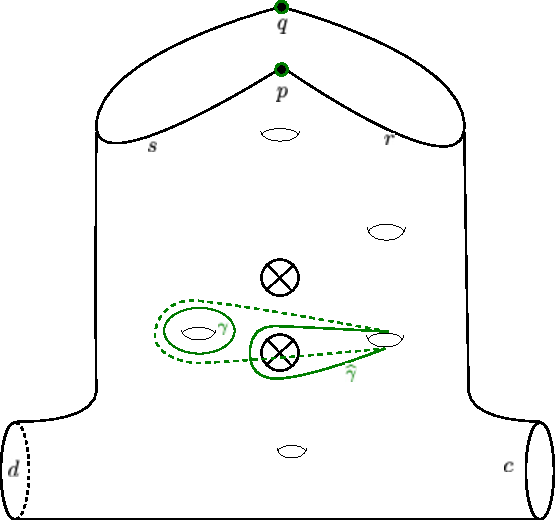
\includegraphics[scale=0.75]{gamma}
    \caption{The curves $\gamma$ and $\widehat{\gamma}$ bound an a non-orientable surface of genus 1.}
    \label{fig:gammacurves}
\end{figure}

\begin{prop}
\label{lem:genus3}
Let $M_{n,k}$ be the mapping torus of $f_{n,k}$. Let $\mathcal{K}_{n,k}$ denote the fibered cone of
$H^1(M_{n,k};\mathbb{R})$ corresponding to the map $f_{n,k}$. 
There is a relatively orientable incompressible surface $F_{n,k}$ embedded in $M_{n,k}$ that is homeomorphic to $\mathcal{N}_3$.
Moreover $F_{n,k}$ is transverse to the suspension flow direction given by $f_{n,k}$ and the Poincar\'e dual of $F_{n,k}$ is in
the closure $\overline{\mathcal{K}_{n,k}}$.
\end{prop}
\begin{proof}
  Let $\gamma \subset T_{0,0}$ be the curve shown in \autoref{fig:gammacurves}. Note that $\gamma$ and $\Phi(\gamma)$ bound a non-orientable surface
  $\widehat{F}$ of genus 1 with boundary. For convenience, we will denote $\Phi(\gamma)$ by $\widehat{\gamma}$. We are going to follow the image of $\gamma$
  under powers of $f_{n,k}$.  Then we attach annuli to the
  boundary of $\widehat{F}$ to obtain $\mathcal{N}_3$. Since $\gamma$ is disjoint from all curves in $\overline{\mathcal{R}}$ and $\overline{\mathcal{B}}$ (as seen in \autoref{fig:curves}), the maps $\Phi_r$ and $\Phi_b$ act trivially on $\gamma$.  Recalling that $f_{n,k}=\rho_2\circ\Phi\circ\Phi_b\circ\Phi_r$, we have the following:
  \begin{align*}
    f_{n,k}(\gamma) &= \rho_2 \circ \Phi \circ \Phi_b \circ \Phi_r(\gamma) \\
                    &= \rho_2 \circ \Phi(\gamma) \\
                    &= \rho_2(\widehat{\gamma}) %\\
   % f^2_{n,k}(\gamma) &= \rho_2^2(\widehat{\gamma}) \\
%                      &\vdots \\
 %   f^k_{n,k}(\gamma) &= \rho_2^k(\widehat{\gamma})\\
  %                    &= \widehat{\gamma}.
  \end{align*}
  It follows that for all $1\leq i\leq k$, the curve $f_{n,k}^i(\gamma)$ is $\rho_2^i(\widehat{\gamma})$.  
  For $1\leq i\leq k$, let $A_i$ be an annulus in $M_{n,k}$ that connects $f_{n,k}^{i-1}(\gamma)$ to $f_{n,k}^i(\gamma)$ obtained by following the suspension
  flow of $f_{n,k}$ around $M_{n,k}$. We can now construct the embedded surface $F_{n,k}$ by taking the union of
  $A_1,A_2,\dots,A_k$ and $\widehat{F}$. Since each $A_i$ has Euler characteristic 0 and the union of $\widehat{F}$ with $A_1,A_2,\dots, A_k$ has empty boundary we see $F_{n,k}$ is homeomorphic to $\mathcal{N}_3$.

 % The resulting surface is an embedded non-orientable surface in a non-orientable $3$-manifold, so we have
 % relative orientability by Proposition \ref{prop:relative-orientability}.

We now need to show that $F_{n,k}$ is relatively orientable. We construct a outwards pointing normal vector field by gluing together the outwards pointing vector field on $\widehat{F}$ and the vector field on the annulus given by following $\gamma$ along the suspension flow.
In general, one cannot glue together such vector fields without making it vanish somewhere, but we control how $\widehat{F}$ and the annulus intersect: namely at the two boundary components of $\widehat{F}$, which are $\gamma$ and $\widehat{\gamma}$.
Choose the outward direction over $\widehat{F}$ to be the forward flow direction.
Construct the outward direction over the annulus by constructing an outward vector field over $\gamma$: we define this to be the vector field that points into the surface $\widehat{F}$.
We then pushforward this vector field in the flow direction; as a result of this, the vector field over $\widehat{\gamma}$ points away from the surface $\widehat{F}$.
This follows from the fact that the homeomorphism $f_{n,k}$ maps the intersection of the tubular neighbourhood of $\gamma$ and $\widehat{F}$ to the intersection of the tubular neighbourhood of $\widehat{\gamma}$ and the complement of $\widehat{F}$.
As a result of this, one can glue together the two non-vanishing vector fields over $\widehat{F}$ and thus annulus to a non-vanishing vector field over the surface $F_{n,k}$, proving the relative orientability of this surface.

% Since $F_{n,k}$ is a non-orientable surface embedded in a non-orientable manifold $M_{n,k}$, Proposition \ref{prop:relative-orientability} tells us that $F_{n,k}$ is relatively orientable (in $M_{n,k}$).

  The proof that $F_{n,k}$ can be isotoped to be transverse to the suspension flow is the same as the
  proof Yazdi uses \cite{yazdi2018pseudo}, which is a restatement of that of Leininger--Margalit \cite{leininger2013number}. We include it here for completeness.  
  
  Let $N(\gamma)$ be a tubular neighborhood of $\gamma$ in $\widehat{F}$.  Let $\eta: \widehat{F} \xrightarrow{} [0,1]$ be a smooth function supported on $N(\gamma)$ with the following properties:
  \begin{itemize}
      \item $\eta^{-1}(1) = \gamma$ and
      \item the derivative of $\eta$ vanishes on $\gamma$. 
    \end{itemize}
    %For each $t\in\RR$, let $\psi_t: M_{n,k}\times S^1 \xrightarrow{} M_{n,k}\times S^1$ be the suspension flow of the map $f_{n,k}$ that snds $(x,t_0)$ to $(x,t_0+t)$. 
Let $\pi:M_{n,k}\rightarrow S^1$ be the projection map and let $t_0$ be such that $\widehat{F}\subset\pi^{-1}(t_0)$.  Let $g: \widehat{F} \xrightarrow{} M_{n,k}$ be the suspension flow of $f_{n,k}$ defined as $g(x) =(x,t_0+k\cdot\eta(x))$. Then the restriction of $g$ to the interior of $\widehat{F}$ is an embedding into $M_{n,k}$ and $g(\gamma) = \widehat{\gamma}$. Therefore the image of $\widehat{F}$ under $g$ is an embedded non-orientable surface of genus three. Moreover, $g(\widehat{F})$ is isotopic to the natural embedding of $F_{n,k}$ in $M_{n,k}$, and is transverse to the suspension flow.  
  %The proof goes through even in this setting essentially because of the local nature of the proof. 
  Therefore, the Poincar\'e dual of $F_{n,k}$ is in $\overline{\mathcal{K}_{n,k}}$ by \autoref{thm:classifying-fibrations}.
   
  Finally, $F_{n,k}$ is incompressible in $M_{n,k}$ because $M_{n,k}$ is hyperbolic, and $F_{n,k}$ is genus $3$, the
  lowest possible genus for a hyperbolic non-orientable surface.
\end{proof}



\p{Step 5: Filling in the Gaps}
Recall that the family of surfaces $P_{n,k}$ that we have constructed have genera in the set $\{(14k-2)n+2\}$.
We now want to construct surfaces of genera not in the set $\{(14k-2)n+2\}$ and pseudo-Anosov homeomorphisms of those surfaces that have small stretch factors.  To do this we use the mapping torus $M_{n,k}= (P_{n,k},f_{n,k})$. Recall from Proposition \ref{lem:genus3} that there exists a relatively incompressible surface $F_{n,k}$ in $M_{n,k}$ that is homeomorphic to $\no_3$.  Let $P_{n,k}^r$ be the oriented sum of $P_{n,k}$ and
$rF_{n,k}$, as defined in Proposition $\ref{thm:oriented-sum}$.  The surfaces $P_{n,k}^r$ will be surfaces of the remaining genera.

\begin{lem}
  The surface $P^r_{n,k}$ is of genus $g^r_{n,k} = g_{n,k} + r$. In particular, as $r$ varies between
  $0$ and $14n$, the genera of $\{P^r_{n,k}\}$ spans the range between $g_{n,k}$ and $g_{n,k+1}$. Moreover,
  $P^r_{n,k}$ is isotopic to a fiber of a fibration of $M_{n,k}$ with pseudo-Anosov monodromy that fixes $2n$
  of the singularities of its invariant foliation.
\end{lem}

\begin{proof}
  The Euler characteristic of an oriented sum is the sum of the Euler characteristics of the summands:
  \begin{align*}
    \chi(P^r_{n,k}) &= \chi(P_{n,k}) + r\cdot\chi(F_{n,k}) \\
                    &= (-2g_{n,k} + 2)-2r \\
                    &= -2(g_{n,k} + r) + 2.
  \end{align*}
  Since $P_{n,k}^r$ has no boundary or punctures, we have that the genus of $P_{n,k}^r$ is $g_{n,k}+r$.

  By Lemma \ref{lem:genus3} we know that $F_{n,k}$ is incompressible and transverse to the suspension flow of given by $f_{n,k}$.  Therefore by Proposition \ref{prop:asymptotic}, there is a pseudo-Anosov homeomorphism of $P_{n,k}^r=P_{n,k}+rF_{n,k}$.
  %with stretch factor at most $\lambda_{n,k}$.
  %\becca[inline]{This sentence is irrelevant to the lemma at hand, right?}
  %\sayantan[inline]{The stretch factor bit is irrelevant, the the fact that the monodromy is pA is not.}
  % Therefore Proposition \ref{thm:oriented-sum} gives us that $P^r_{n,k}$ is isotopic to a fiber of a fibration of $M_{n,k}$. Let $f^r_{n,k}$ be the first return map of the new fibration of $M_{n,k}$ over $P^r_{n,k}$.  Since $f_{n,k}$ is a pseudo-Anosov monodromy of $M_{n,k}$, we have that $M_{n,k}$ is hyperbolic.  Therefore all monodromies of $M_{n,k}$ are pseudo-Anosov.  In particular $f^r_{n,k}$ is a pseudo-Anosov homeomorphism of $P_{n,k}^r$.

 As in Yazdi \cite[Lemma 3.5]{yazdibounds}, $f_{n,k}$ fixes the $2n$ singularities of the stable foliation that are the intersection points of the axis of $\rho_1$ with
  $P_{n,k}$. By Lemma \ref{lem:genus3}, the surface $F_{n,k}$ can be isotoped to be transverse to
  the suspension flow and disjoint from the orbit of the $2n$ singularities of $f_{n,k}$.  Hence the monodromy
  $f^r_{n,k}$ still fixes the corresponding $2n$ singularities on $P^r_{n,k}$.
\end{proof}

We now prove the non-orientable version of the final piece of Yazdi's proof \cite[Lemma 3.6]{yazdi2018pseudo}.
\begin{lem}
\label{lem:bound}
Let $\lambda_{n,k}^r$ be the stretch factor of $f_{n,k}^r:P_{n,k}^r\rightarrow P_{n,k}^r$. Then there exists a constant $C > 0$ such that for every $n \geq 1$, $k \geq 3$, and $0 \leq r \leq 14n$ we have the following upper bound on $\log(\lambda_{n,k}^r)$:
\begin{align*}
  \log(\lambda^r_{n,k}) \leq C\frac{n}{g^r_{n,k}}.
\end{align*}
\end{lem}
\begin{proof}
  Let $\mathcal{K} = \mathcal{K}_{n,k}$ be the fibered cone in $H^1(M_{n,k};\mathbb{R})$ corresponding to $f_{n,k}$ and $h: \mathcal{K} \xrightarrow[]{} \mathbb{R}$
  the function described in \autoref{thm:fm}. Note that $g_{n,k}\geq 42$, therefore we have the following bounds on $g_{n,k}^r$:
  \begin{align*}
    g^r_{n,k} &= g_{n,k} + r \\
              &\leq g_{n,k} + 14n \\
              &< 2g_{n,k}.
  \end{align*}
  Let $\omega$ be the Poincar\'e dual of $P^r_{n,k}$ and $\alpha$ the Poincar\'e dual of $P_{n,k}$.  Then the following string of inequalities holds:
  \begin{align*}
    h([\omega]) &< h([\alpha]) &&\text{(Convexity of $h$)}\\
                &\leq C'\frac{n}{g_{n,k}} &&\text{(Lemma \ref{lem:upperbound})}\\
                &\leq 2C'\frac{n}{g^r_{n,k}}&&\text{(upper bound for $g_{n,k}^r$)}. 
  \end{align*}
\end{proof}

%Each surface $P^r_{n,k}$ is isotopic to a fiber of fibration of $M_{n,k}$ and has a pseudo-Anosov monodromy with a bounded stretch factor.

In the initial construction of $P_{n,k}$, there were $2n$  marked points, which were singularities of the map $f_{n,k}$.  By the construction of $P_{n,k}^r$, these marked points are also singularities of $f^r_{n,k}$.  Now we puncture $P_{n,k}^r$ at $n$ of these marked points.  We could think of this as removing all copies of the point $p$ in the construction of $P_{n,k}$ in step 1. %as a map on a non-orientable surface of genus $g^r_{n,k}$ with $n$ punctures. Also note from above weknow $g^r_{n,k}$ covers all natural numbers between $g_{n,k}$ and $g_{n,k+1}$, thus this set of genera for all $r$ covers all natural numbers larger than $g_{n,3} = 40n + 2$. 

We can now give a proof of \autoref{thm:stretch1}.

%\begin{manualtheorem}{\ref{thm:stretch1}}
%For any fixed $n \in \mathbb{N}$, there are positive constants $B'_1 = B'_1(n)$ and $B'_2 = B'_2(n)$ such that for any $g \geq 2$, the stretch factor satisfies the following inequalities.
 % \begin{align*}
  %  \frac{B'_1}{g} \leq l'_{g,n} \leq \frac{B'_2}{g}
  %\end{align*}
%\end{manualtheorem}
\begin{proof}[Proof of \autoref{thm:stretch1}]
As above, the lower bound follows easily from the lower bound in the orientable setting.  % as demonstrated in the discussion following the initial statement of \autoref{thm:stretch1}. For ease of reading, we replicate that here.  
 % Let $f$ be the pseudo-Anosov map with the minimal stretch factor on $\no_{g,n}$. Let $\wt{f}:\os_{g-1, 2n}\rightarrow\os_{g-1,2n}$ be the orientation preserving lift of $f$ to the orientation double cover of $\no_{g,n}$. By Proposition \ref{prop:2}, $\wt{f}$ has the same stretch factor as $f$. The former is bounded below by $\frac{B}{g}$, and thus the stretch factor of $f$ is bounded below as well.
  
  To find the upper bound, let $C'=\frac{C}{2}$ be the value given in Lemma \ref{lem:bound}. Let $B'_2(n)$ be the
  following quantity:
  \begin{align*}
    B'_2(n) = \max\{2C'n, \ell'_{1,n}, 2\ell'_{2,n}, \dots, (40n + 1)\ell'_{40n+1,n}\}
  \end{align*}
  By Proposition \ref{prop:asymptotic} and Lemma \ref{lem:bound}, $B'_2(n)$ is an upper bound for $g\cdot \ell'_{g,n}$.
\end{proof}